\documentclass[11pt]{article}

\usepackage{graphicx}

\newcommand{\numpy}{{\tt numpy}}    % tt font for numpy
\topmargin -1in
\textheight 9in
\oddsidemargin -.25in
\evensidemargin -.25in
\textwidth 7in

\begin{document}

% https://moodle.up.pt/mod/assign/view.php?id=72723
\author{Miguel Sozinho Ramalho, UP201403027}
\date{March $6^{th}$, 2019}
\title{Algorithms for Bioinformatics: Project 1\\Definition of Python Class for Sequence Manipulation}
\maketitle

% \medskip

\section{Introduction}
The current report describes a practical approach for creating a Python3 library capable of handling and manipulating information on biological sequences. It is considered paramount that Deoxyribonucleic acid (DNA), Ribonucleic acid (RNA) and Protein (collection of Aminoacids) sequences can be represented and modified. The tool should be able to perform typical operations on those sequences in an efficient manner. Contextualizing, this project belongs to the course of Algorithms in Bioinformatics.
% Contextualizar e descrever brevemente o problema.

\section{Implementation}
The main challenge of this project is the architecture design. Namely, how to devise the tool in a way that allows for adding new features, representing the real world structure of the aforementioned sequences while making the most out of Python's design and syntax. 

Although an initial approach was conceived with a single class, it quickly became obvious that it was prone to bugs and hardly represented the real world organization. In the end, and following the object-oriented technique studied in classes, an inheritance implementation was designed consisting of a main class \textbf{BioSeq} and three direct child classes \textbf{DNASeq}, \textbf{RNASeq} and \textbf{ProteinSeq}. 

The mother class contains all the functionality that is applicable to every descendant and each child individually implements the methods that are class specific. Additionally, functions that were abstract and not specific to a class instance were isolated in a \textbf{utils} module.

Due to Python's flexibility in handling object attributes it was decided that no \textbf{set} methods would be implemented, giving some freedom of usage to the user; it was also decided that all the necessary assertions and checks would be done on the initialization methods of each class. However, the assertion methods should also be accessible by the user to validate any new changes. Also, it was decided that empty sequences are considered valid, otherwise the tool would be too strict and not user friendly.

In order to guarantee a good quality of the tool, it was required to write unit tests for all the developed methods (see Figure \ref{fig:coverageReport} for the 100\% coverage) and to document every implemented feature. 
% Descrição e estratégias de implementação - Discutir abordagens relevantes ao problema.


\section{Results}
Of the required features, all were implemented, namely:
\begin{itemize}
    \itemsep0em 
    \item Class constructor with sequence and sequence type (\textbf{\_\_init\_\_})
    \item Methods for visualizing class information (\textbf{\_\_str\_\_}, \textbf{pretty\_print})
    \item Sequence validation (\textbf{\_assert\_valid\_sequence}, \textbf{\_assert\_seq\_type})
    \item Symbol/Token frequency (\textbf{frequency})
    \item GC content (\textbf{gc\_content})
    \item Reverse complement (\textbf{reverse\_complement})
    \item Transcription (\textbf{transcription})
    \item Translation (\textbf{translation})
    \item Codon usage (\textbf{codon\_usage})
    \item Open Reading Frames (ORFs) by minimum size (\textbf{\_reading\_frames}, \textbf{open\_reading\_frames})
    \item Pretty-printing of some instance information (\textbf{pretty\_print})
    \item Input and Output from/to a file (\textbf{save}, \textbf{load})
    \item Reading FASTA files (\textbf{utils.read\_fasta})
\end{itemize}

Besides the baseline features, some were also implemented, namely:
\begin{itemize}
    \itemsep0em 
    \item Implementation of special python methods to better handle the sequences (\textbf{\_\_str\_\_}, \textbf{\_\_repr\_\_}, \textbf{\_\_len\_\_}, \textbf{\_\_getitem\_\_}, \textbf{\_\_getslice\_\_})
    \item Extra method that uses Regular Expressions to validate sequences \textbf{\_assert\_valid\_sequence\_regex}
    \item performance concerns when designing the methods (use of hashmaps, generators, saving as little information on the files as possible, avoid using unnecessary RAM, and others)
    \item Documentation and testing of all the methods
\end{itemize}
\begin{figure}[h!]
    \centering
    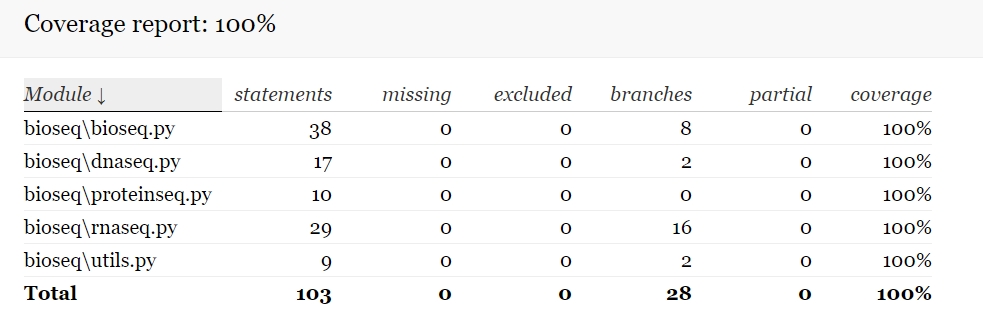
\includegraphics[width=0.65\textwidth]{coverageReport.png}
    \caption{Automatically generated test coverage report for the developed Python module}
    \label{fig:coverageReport}
\end{figure}

The documentation can be seen by opening the file \textit{docs/\_build/html/index.html} in an external browser or by typing \textbf{help(bioseq.moduleName)} on the Python console for the desired module. 

% Deve indicar que funcionalidades foram implementadas, se conseguiu implementar todas as funcionalidades pedidas e se implementou outras funcionalidades além das especificadas.

\section{Conclusions}
Looking back at all the progress made with this project, the author concludes there was a lot learned and also that most concepts became clearer when they had to be organized so meticulously, as in the current tool. It is his belief that the work produced is of sufficient quality to be used in future projects and also to be extended as more relevant bioinformatics techniques are learned.
% Comentários e Conclusões.

\section{References}
\textit{(No paper references required and all other mentions like Python, FASTA, DNA, RNA, Aminoacid, OOP, and others are considered base knwoledge prior to reading this document)}
%  (precisam ser explicitamente citadas no texto para saberem de onde o texto foi retirado/adaptado! Copiar é crime e poderá transformar-se em processo disciplinar, portanto evitem copiar textos e códigos. Se utilizarem figuras retiradas da web ou de livros ou de artigos etc, é necessário colocar uma referência explícita e clara. Por favor tenham atenção aos erros ortográficos.


\end{document}
\grid
\grid